\section{Introduction}
In the initial years of the 60s,computers required giant rooms and consumed giant amounts of electricity, had dear electronic elements and made little or no process output.However,smaller computers eventually replaced those room-size computers.At the top of the last century,the magnitude of computing and infra- structure node organized to make a distributed system, that provided a rise in efficiency. In recent years,when the demand of information and on line users has immensely in- rumpled,the ancient computing infrastructure is turning into costlier and tougher to manage.Traditional computing is not suitable for accessing knowledge any wherever and at anytime.In order to try to to therefore, we'd like to save lots of the info on Associate in Nursing auxiliary storage system.Ad- ditionally, the rise of on-line users on networking sites, online surfing, video conferencing,and such can not be handled by ancient computing.
Distributed computing is one amongst the foremost blazing center specialised subjects within the advanced time. it's developed with expansive going impacts crosswise over IT, organizations, programming building and data stockpiling. one amongst the principle impacts is that the growth of their ability. This increase in capability does not essentially mean a rise in expenses in hardware, software, and coaching of private to mention many. in keeping with the National Institute of Standards and Technology (NIST) definition, the cloud computing could be a model for facultative convenient, resource pooling, ubiquitous, on-demand access which can be simply delivered with differing types of service supplier interaction. The cloud computing follows easy pay as you go (PAYG) model, wherever you get the services youve used. One of the main edges of PAYG model is that we are able to cut back our expenditure by provisioning a particular amount of resources. The user will choose processor, memory, hard disk, software package, networking, access management and any extra new package PRN to their setting. The resources provided on-demand to the client or finish users. It provides tremendous edges to business and residential users and attracts the eye of the analysis community Cloud computing implements virtualization technique is to produce resources with efficiency to the tip user. The characteristics of cloud computing include tractableness, quantifiability, and handiness. additionally, cloud computing is additionally economical, on-demand service, expedient, ubiquitous, multitenant, elasticity, and stability. Cloud computing offers mainly 3 service delivery models; Infrastructure as a Service (IaaS), Platform as a Services (PaaS)
and software system as a Service (SaaS). office defines four-development model of the cloud: public, private, hybrid and community. Cloud computing uses cloud server stack wherever the shopper or user is on the front end and server on the rear finish. Services reside in middleware of stack as shown in Fig. 1. At the top level resides the appliance, that directly delivers the outsourced software system to the shopper and eliminates sophisticated software system. Customers do no got to expend cash to put in software system, solely they obtain their usage.\begin{figure}
	\centering
	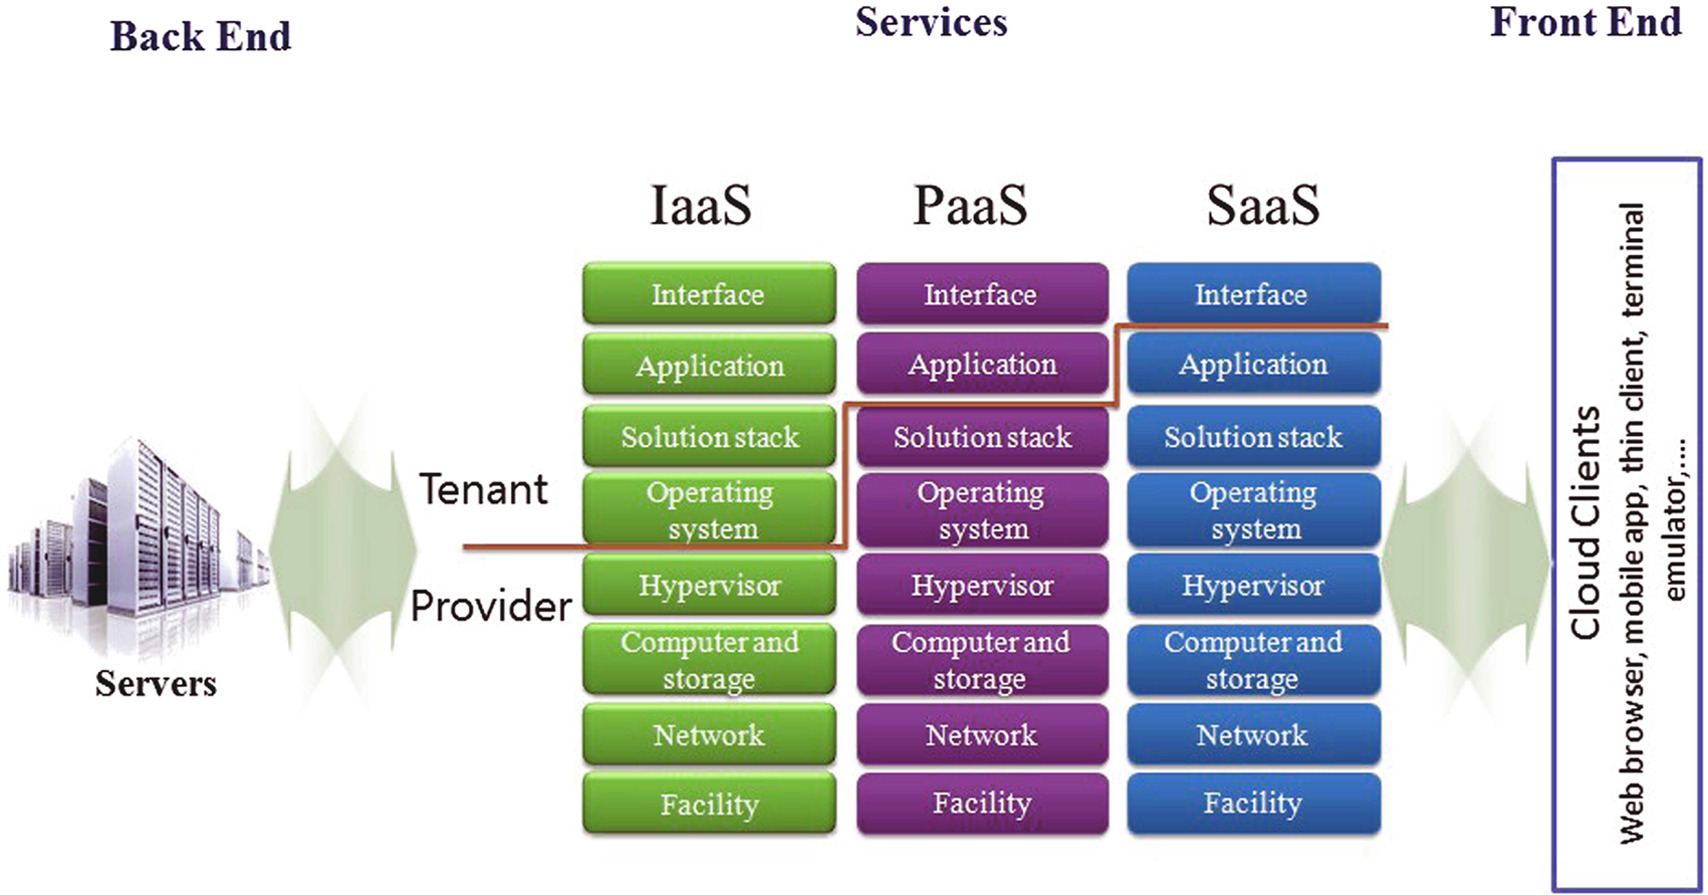
\includegraphics[width=\linewidth]{cloud.jpg} 
	\caption{Cloud service delivery models}
	\label{fig:cloud}
\end{figure}


NIST is accountable for developing tips and standards to produce security in cloud atmosphere.Here we have a tendency to outline the cloud design as a fourfold, that consists of: (a) cloud computing concept and characteristics (b) cloud deployed models (c) cloud service delivery models (d) cloud security concept. the small print of the cloud design ar given below:

\section{Cloud service delivery models}
the major 3 delivery models ar IaaS, PaaS, and SaaS. Still several service models ar accessible as per their practicality and repair providing capabilities, that have LED to the creation of Anything as service AaaS delivery models. during this section, we have a tendency to discuss the various styles of service models as shown

\textit{Infrastructure as a service (IaaS)} It belongs to all-time low of the model. IaaS deals with pc hardware (network storage, virtual server/machine, knowledge center, processor, and memory) as a service. IaaS supports the revolution within the business investment in IT infrastructure The snap of allocating physical or virtual resources helps providing the infrastructure in associate degree abstract manner. It additionally provides scalability and provisions (such as hypervisor) problems with infrastructure while not the requirement of paying huge quantity of funds and time.


\textit{Platform as a service (PaaS):} it is in middleware of service model and it delivers the services in the form of development tools, framework, design, programs, and Integrated Development Environments(IDE). In alternative words, the purchasers area unit ready to management the
applications however do not have any means to manage the underlying infrastructure. It will be useful in things wherever multiple developers located in several physical locations ought to work along. a well-liked PaaS supplier is Google App
Engine. it's a software package Development Kit (SDK) that provides associate
degree atmosphere that supports Python, Java, and Go programming languages. because it provides options that area unit prepared for the client, PaaS is more extensile and additional versatile than SaaS model.

\textit{Software as a service (SaaS)}  (SaaS) it is a set of remote computing services. SaaS is at the highest model among the delivery models. It permits the applications to deploy remotely by third-party vendors. It allows the client to use cloud service provider’s application (CSP’s) running on cloud infrastructure
via the web. SaaS is that the prevailing cloud market and still keeps growing quickly. Google App and Salesforce area unit samples of SaaS suppliers.

\begin{figure}[h]
	\centering
	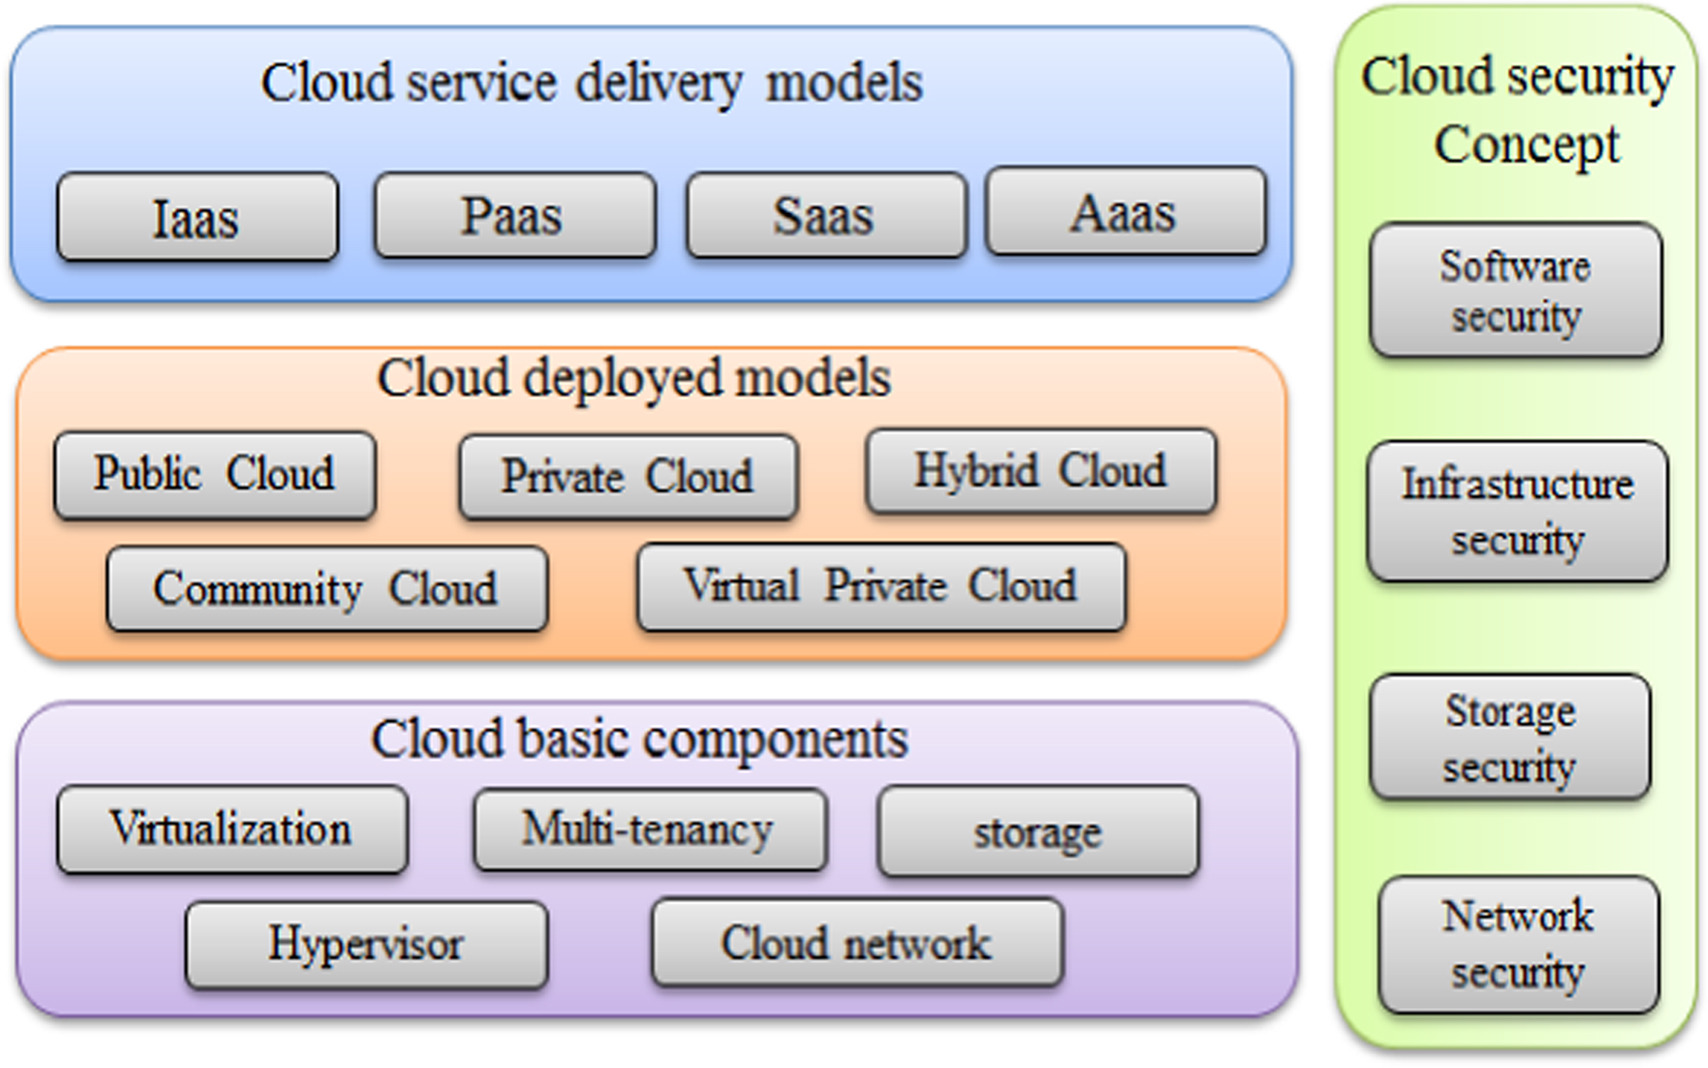
\includegraphics[width=\linewidth]{ServiceModels.JPG}
	\caption{Cloud computing framework}
	\label{fig:service-models}
\end{figure}


\textit{Anything as a service (AaaS)} it is a collective term which mixes variety of things as X as a service. X is also something or everything as a service. This service becomes interchangeable in cloud landscape. The cloud system area unit ready to support the massive resource to specific, personal and granular necessities mistreatment Monitor as a Services (MaaS), knowledge as a
Service (DaaS), Communication as a Service (CaaS), Security as a Service (SecaaS), Routing as a Service (RaaS).


\section{Cloud deployed models}
Cloud computing typically depends on shared resources by native servers or individual devices. Therefore, it is able to come through consistency by taking the advantage of resource sharing. Deployed model tells what is the aim and nature of the cloud. By doing this, it reduces the facility of servers, capital expenditure and management the disbursal. bureau defines 5 styles of deployed models:

•\textit{ Private cloud}: Cloud computing operates and manages inside the info center of a corporation is called a personal cloud. several shoppers of cloud infrastructure (eg, business units) are together with provision for exclusive use by one organization. in an exceedingly personal cloud, it is abundant easier to spot the customer and merchant relationship as a result of the infrastructure in hand and operated by constant organization. Therefore, security risks area unit easier to notice.

•\textit{Public cloud:} it is truth illustration of cloud hosting wherever the client and supplier have a strong Service Level Agreement (SLA) to take care of the trust between them. during this cloud infrastructure, open access to the general public and organization provided. Businesses, academics, or governmental organizations own public cloud environments. this suggests multiple entities could own and operate a public cloud. This creates several problems, as we tend to dont recognize wherever the resources area unit settled or World Health Organization owns them, increasing the issue of protective them from attack.

\textit{Community cloud:} Cloud infrastructure of the organizations shared considerations(mission, security necessities,policy, and compliance considerations) of shoppers a special provision has been created for exclusive use by the community model. it is in hand, managed, and community organizations, a third party, or some combination of them is driven by one or additional, which could also be gift on or off field. In easy words, a community cloud is being shared and controlled by multiple organizations.

\textit{Hybrid cloud:} it is the mix of 2 or additional clouds (public, private, community). Usually, the data and application area unit sure along by standardized and behaviour technology. Hybrid cloud offers the advantages of various clouds readying models. However, it is well organized and safer than public cloud whereas accessing the entities over the net.

\textit{Virtual private cloud:} It is a semi-private cloud, which is fewer resources, and it consists of virtual private network (VPN). It is on demand configurable pool of shared resources allocated within the cloud environment.

\section{Cloud computing basic component}
 
 In this section, we will discuss the fundamental parts on that cloud computing deployed. These components incorporates a large vary of services that we are able to use everywhere the net. Here we have a tendency to discuss some vital component:
 
 \textit{ Virtualization:} It plays a vital role in deploying the cloud. it is the strategic part in the cloud, that permits the physical resources by multiple shoppers. It creates the virtual instance of resource or device like software system, servers, network resources and storage devices whereby the framework utilize the resources into quite one execution surroundings.
 
 \textit{ Multi-tenancy:} Multi-tenant surroundings will have multiple customers or users who doesn't see or share every other’s knowledge however will share resource or application in Associate in Nursing execution surroundings, although they
 may not belong to identical organization. Multi-tenancy results the optimum utilization of hardware and data storage mechanism.
 
 \textit{Cloud storage:} It is a component, which maintained, managed, and backed up remotely and it made available over the network where the users can access data.

 \textit{The hypervisor:} The thus referred to as virtual machine monitor or manager could be a key module of virtualization. It permits multiple Virtual Machines (VMs) to run on one hardware host. It manages and monitors the various in operation systems, that run in a very shared physical system.
 
 \textit{Cloud Network:} It will operate quite one standard knowledge centers, a typical knowledge center contains hundreds or thousands of servers. To expeditiously build and manage the storages the cloud needs a secure network infrastructure referred to as cloud networking. It needs an online affiliation and similar with a virtual personal network that permits the user to firmly access printers, applications, files etc.






